\documentclass{beamer}
\usepackage[utf8]{inputenc}
\usepackage[spanish]{babel}
\usepackage{hyperref}
\usepackage{verbatim}
\usepackage{listings}
\usepackage{tikz}
\usetikzlibrary{arrows}

\setbeamercovered{invisible}
\usetheme{Frankfurt}
\usefonttheme{serif}

% Configurar los listings (Códigos)
\renewcommand{\lstlistingname}{Código}
\lstset{
	language=C++,               % Lenguaje
	basicstyle=\ttfamily\footnotesize,  % Tipo de fuente
	keywordstyle=\color{blue},  % Color de palabras clave
	stringstyle=\color{red},    % Color de strings
	commentstyle=\color{gray},  % Color de comentarios
	showstringspaces=false,     % No muestrar el _ cuando el string tiene espacios
	breaklines = true,          % Partir las líneas largas
	breakatwhitespace=true,	    % Partir las líneas en un espacio
	numbers=left,				% Numerar las líneas a la izq
	numberstyle=\tiny,			% Poner los números de las líneas pequeños
	numberblanklines=true,      % Numerar las líneas en blanco
	columns=fullflexible,       % No perder el formato al dejar los espacios
	keepspaces=true,   			% Dejar los espacios insertados
	frame=tb,					% Poner el recuadro
}

% Poner una diapositiva con el nombre de la sección cuando esta inicia
\AtBeginSection[]{
  \begin{frame}<beamer>
    \frametitle{Contenido}
    \tableofcontents[sectionstyle=show/hide,subsectionstyle=hide/show/hide]
  \end{frame}
  \addtocounter{framenumber}{-1}% If you don't want them to affect the slide number
}

% Configuración del paquete tikz para los grafos
\pgfdeclarelayer{background}
\pgfsetlayers{background,main}

\tikzstyle{vertex}=[circle,fill=black!25,minimum size=20pt,inner sep=0pt]
\tikzstyle{edge} = [draw,thick,->]
\tikzstyle{weight} = [font=\small]
\tikzstyle{selected edge} = [draw,line width=4pt,->,>=stealth',shorten >=11pt, red!50]

\title{Semillero de Programación}
\subtitle{Algoritmo de máximo flujo}
\author{Ana Echavarría \and Juan Francisco Cardona}

\institute{Universidad EAFIT}
\date{3 de mayo de 2013}

\begin{document}

\begin{frame}
	\titlepage
\end{frame}

\begin{frame}
	\frametitle{Contenido}
	\tableofcontents
\end{frame}

\section[Problemas]{Problemas semana anterior}
	\subsection{Problema A - I love strings!}
	
	\begin{frame}
		\frametitle{Problema A - I love strings!}
		\begin{itemize}
			\item Hay que hallar rápidamente si un string $s$ aparece en un string $t$.
			\item Utilizar kmp y retornar verdadero o falso dependiendo de si se encontró el string o no.
		\end{itemize}
	\end{frame}
	
	\begin{frame}[fragile, allowframebreaks]
		\frametitle{Implementación}
		\begin{lstlisting}
			bool kmp(const string &needle, const string &haystack){
			   int m = needle.size();
			   vector<int> border(m);
			   border[0] = 0;

			   for (int i = 1; i < m; ++i) {
			      border[i] = border[i - 1];
			      while (border[i] > 0 and needle[i] != needle[border[i]])
			         border[i] = border[border[i] - 1];
			      if (needle[i] == needle[border[i]]) border[i]++;
			   }

			   int n = haystack.size();
			   int seen = 0;
			   for (int i = 0; i < n; ++i){
			      while (seen > 0 and haystack[i] != needle[seen])
			         seen = border[seen - 1];
			      if (haystack[i] == needle[seen]) seen++;
			      if (seen == m) return true;
			   }
			   return false;
			}

			int main(){
			   int cases; cin >> cases;
			   while(cases--){
			      string haystack; int q;
			      cin >> haystack >> q;
			      while (q--){
			         string needle; cin >> needle;
			         if (kmp(needle, haystack)) puts("y");
			         else puts("n");
			      }
			   }
			   return 0;
			}
		\end{lstlisting}
	\end{frame}
	
	\subsection{Problema B - Power strings}
	\begin{frame}[fragile]
		\frametitle{Problema B - Power strings}
		\begin{itemize}
			\item Un string $s$ de tamaño $n$ se dice que tiene periodo $k$ si $s(x + k) = s(x)$ $\forall x : x + k < n$
			\item Notemos que el mínimo $k$ que cumpla esa propiedad es \verb|n - border[n-1]|
			\item Este $k$ es mínimo porque \verb|border[n-1]| es máximo
		\end{itemize}
	\end{frame}
	
	
	\begin{frame}[fragile]
		\frametitle{Problema B - Power strings}
		\begin{itemize}
			\item En el problema nos interesa que el mínimo periodo (prefijo de tamaño $k$) aparezca un número entero de veces en la cadena
			\item Para comprobar esto último basta con ver que $n$ sea divisible por $k$
			\item Si $n$ no es divisible por $k$ entonces el mínimo periodo no aparece un número entero de veces y la respuesta es 1.
		\end{itemize}
	\end{frame}
	
	\begin{frame}[fragile, allowframebreaks]
		\frametitle{Implementación}
		\begin{lstlisting}
			const int MAXN = 1000005;
			int border[MAXN];

			int main(){
			   ios::sync_with_stdio(false); // Para hacer la I/O mas rapido
			   // Con esa línea ya sólo se puede usar cin y cout si no el programa se enloquece con la entrada y la salida
			   string s;
			   while (cin >> s){
			      if (s == ".") break;
			      int n = s.size();

			      border[0] = 0; 
			      for (int i = 1; i < n; ++i) {
			          border[i] = border[i - 1];
			          while (border[i] > 0 and s[i] != s[border[i]]) {
			              border[i] = border[border[i] - 1];
			          }
			          if (s[i] == s[border[i]]) border[i]++;
			      }

			      int base = n - border[n-1];
			      if (n % base == 0) cout << n / base << endl;
			      else cout << 1 << endl;
			   }
			    return 0;
			}
		\end{lstlisting}
	\end{frame}

\section{Motivación}

	\begin{frame}
		\frametitle{Red de flujos}
		\begin{itemize}
			\item De igual manera como se puede crear un grafo para modelar rutas y hallar la mínima distancia entre dos lugares, se pueden usar grafos para representar una \textbf{red de flujos}.
			\item Acá los nodos son lugares a los que hay que transportar material y los pesos de cada arista es la \textbf{tasa máxima} a la cual ese material fluye entre los nodos.
			\item Algunos ejemplos en las que las redes de flujos se usan para modelar problemas son: líquido que fluye por tuberías, corriente eléctrica que fluye por un cableado, flujo de producción en una línea de ensamble, etc.
		\end{itemize}
	\end{frame}
	
	\begin{frame}
		\frametitle{Ejemplo}
		\begin{block}{Ejemplo}
			Se tiene un sistema de tuberías unidireccionales que salen desde la planta de tratamientos en la ciudad $s$ y pasan por varias ciudades incluida la ciudad $t$. La capacidad máxima de las tuberías (litros/hora) entre cada par de ciudades es conocida. ¿Cuál es la máxima cantidad de agua que puede llegar a la ciudad $t$ en una hora?
		\end{block}
		\begin{figure}
			\begin{tikzpicture}[scale=1.8, auto,swap]
				% First we draw the vertices
				\foreach \pos/\name in {{(0,0.7)/s}, {(1.5,1.4)/1}, {(1.5,0)/2},
										{(3,1.4)/3}, {(3,0)/4}, {(4.5,0.7)/t}}
				\node[vertex] (\name) at \pos {$\name$};
	
				% Connect vertices with edges and draw weights
				\foreach \source/ \dest /\weight in {s/2/13, 2/1/4, 2/4/14, 3/2/9, 4/3/7, 4/t/4}
				\path[edge] (\source) -- node[weight] {$\weight$} (\dest);
			
				\foreach \source/ \dest /\weight in {s/1/16, 1/3/12, 3/t/20}
				\path[edge] (\source) -- node[weight, above] {$\weight$} (\dest);
			\end{tikzpicture}
		\end{figure}
	\end{frame}
	
\section[Max-flow]{Problema de máximo flujo}
	
	\begin{frame}
		\frametitle{Red de flujos}
		\begin{block}{Red de flujos}
			Una red de flujos $G = (V, E)$ es un grafo conexo y dirigido en donde cada arista $(u, v) \in E$ tiene una capacidad \textbf{no negativa} $c(u,v) \geq 0$.\\ \quad \\
			% En una red de flujos es necesario que si $(u, v) \in E$ entonces $(v, u) \not\in E$ \\ \quad \\
			Si $(u, v) \not\in E$ entonces $c(u, v) = 0$ \\ \quad \\
			Se distinguen dos nodos: la fuente $s$ y el sumidero $t$.
		\end{block}
	\end{frame}

	\begin{frame}
		\frametitle{Flujo}
		Sea $G = (V, E)$ una red de flujos con fuente $s$ y sumidero $t$.
		\begin{block}{Flujos}
			Un flujo es una función $f:V \times V \rightarrow \mathbb{R}$ que cumple que:
			\begin{itemize}
				\item \textbf{Restricción de capacidad:}
					$$f(u,v) \leq c(u,v) \,\,\,\, \forall\, u,v \in V$$
				\item \textbf{Simetría:} 
					$$f(u,v) = -f(v,u) \,\,\,\, \forall\, u,v \in V$$
				\item \textbf{Conservación de flujo:} El flujo que sale de un nodo diferente de $s$ y $t$ es igual al que entra al nodo. $\forall\, u \in V - \{s, t\}$ 
					$$\displaystyle\sum_{v \in V}{f(u,v)} = \displaystyle\sum_{\substack{v \in V\\f(u,v) < 0}}{f(u,v)} + \displaystyle\sum_{\substack{v \in V\\f(u,v) > 0}}{f(u,v)} = 0 \,\,\,\, $$
			\end{itemize}
		\end{block}
	\end{frame}

	\begin{frame}
		\frametitle{Problema de máximo flujo}
		Sea $G = (V, E)$ una red de flujos con fuente $s$, sumidero $t$, función de flujos $f$.
		\begin{block}{Definiciones}
			\begin{itemize}
				\item Al valor $f(u,v)$ se le llama flujo del nodo $u$ al nodo $v$.
				\item El valor del flujo de $G$ se denota por $|f|$ y corresponde al flujo que sale de $s$ menos el flujo que entra a $s$ $$|f| = \displaystyle\sum_{v\in V}{f(s,v)}$$
			\end{itemize}
		\end{block}
	
		\begin{block}{Problema de máximo flujo}
			Dados $G$, $s$ y $t$ hallar un flujo de $G$ que tenga valor máximo.
		\end{block}
	\end{frame}
		
		
	\begin{frame}
		\frametitle{Red residual}
		Dados una red e flujos $G = (V, E)$ y un flujo $f$.\\
		La red residual de $G$ dado que se ha ``bombeado'' un flujo $f$ es un grafo $G_f = (V, E_f)$ con una función de costos $c_f$.\\ 
		El peso $c_f$ de una arista $(u, v) \in E_f$ es el valor de flujo que todavía se puede ``bombear'' desde $u$ hasta $v$ sin violar la capacidad de $(u, v)$.\\
		$$c_f(u,v) = c(u,v) - f(u,v)$$\\
	\end{frame}

	\begin{frame}
		\frametitle{Ejemplos}
		\begin{itemize}
			\item Si $c(u,v) = 16$ y $f(u,v) = 11$ entonces $c_f(u,v) = 16 - 11 = 5$. Esto significa que por la arista $(u,v)$ todavía se pueden bombear 5 unidades de flujo sin violar la capacidad.
			\item Si $c(u,v) = 16$ y $f(u,v) = -4$ (es decir que $f(v, u) = 4$) entonces $c_f(u,v) = 16 - (-4) = 20$. Esto significa que por la arista $(u,v)$ no sólo se pueden ``bombear'' las 16 unidades que tiene de capacidad esa arista, sino que también se pueden ``desbombear'' las 4 unidades que se habían bombeado de $v$ a $u$.
		\end{itemize}
	\end{frame}

	\begin{frame}
		\frametitle{Ejemplo}
		Red de flujos: Peso de arista $(a,b)$ es $c(a, b) / f(a, b)$
		\begin{figure}
			\begin{tikzpicture}[scale=1.8, auto,swap]
				% First we draw the vertices
				\foreach \pos/\name in {{(0,0.5)/s}, {(1.5,1)/1}, {(1.5,0)/2},
										{(3,1)/3}, {(3,0)/4}, {(4.5,0.5)/t}}
				\node[vertex] (\name) at \pos {$\name$};
	
				% Connect vertices with edges and draw weights
				\foreach \source/ \dest /\weight in {s/2/{13/4}, 2/4/{14/4}, 3/2/{9/0}, 4/3/{7/0}, 4/t/{4/4}}
				\path[edge] (\source) -- node[weight] {$\weight$} (\dest);
			
				\foreach \source/ \dest /\weight in {s/1/{16/8}, 1/3/{12/8}, 3/t/{20/8}}
				\path[edge] (\source) -- node[weight, above] {$\weight$} (\dest);
			
				\foreach \source/ \dest /\weight in {2/1/{4/4}}
				\path[edge] (\source) -- node[weight, left] {$\weight$} (\dest);
			
			\end{tikzpicture}
		\end{figure}
		% 
		Red residual: Peso de arista $(a,b)$ es $c_f(a,b)/ c_f(b,a)$
		\begin{figure}
			\begin{tikzpicture}[scale=1.8, auto,swap]
				% First we draw the vertices
				\foreach \pos/\name in {{(0,0.5)/s}, {(1.5,1)/1}, {(1.5,0)/2},
										{(3,1)/3}, {(3,0)/4}, {(4.5,0.5)/t}}
				\node[vertex] (\name) at \pos {$\name$};
	
				% Connect vertices with edges and draw weights
				\foreach \source/ \dest /\weight in {s/2/{9/4}, 2/4/{10/4}, 3/2/{9/0}, 4/3/{7/0}, 4/t/{0/4}}
				\path[edge] (\source) -- node[weight] {$\weight$} (\dest);
	
				\foreach \source/ \dest /\weight in {s/1/{8/8}, 1/3/{4/8}, 3/t/{12/8}}
				\path[edge] (\source) -- node[weight, above] {$\weight$} (\dest);
			
				\foreach \source/ \dest /\weight in {2/1/{0/4}}
				\path[edge] (\source) -- node[weight, left] {$\weight$} (\dest);
			\end{tikzpicture}
		\end{figure}
	\end{frame}
	
	\begin{frame}
		\frametitle{Camino de aumentación}
		\begin{block}{Camino de aumentación}
			Dada una red residual $G_f$ un camino de aumentación es un camino simple (sin ciclos) $p$ que va de $s$ a $t$ en $G_f$ tomando solo aristas de peso mayor que 0.\\ \quad \\
			En otras palabras un camino de aumentación es un camino por el cual todavía se puede bombear flujo de $s$ a $t$ en $G$ sin violar las restricciones de capacidad.
		\end{block}
	\end{frame}

	\begin{frame}
		\frametitle{Ejemplo}
		Red de flujos: Valor escrito en arista $(a,b)$ es $c(a, b) / f(a, b)$
		\begin{figure}
			\begin{tikzpicture}[scale=1.8, auto,swap]
				% First we draw the vertices
				\foreach \pos/\name in {{(0,0.5)/s}, {(1.5,1)/1}, {(1.5,0)/2},
										{(3,1)/3}, {(3,0)/4}, {(4.5,0.5)/t}}
				\node[vertex] (\name) at \pos {$\name$};
	
				% Connect vertices with edges and draw weights
				\foreach \source/ \dest /\weight in {s/2/{13/4}, 2/4/{14/4}, 3/2/{9/0}, 4/3/{7/0}, 4/t/{4/4}}
				\path[edge] (\source) -- node[weight] {$\weight$} (\dest);
			
				\foreach \source/ \dest /\weight in {s/1/{16/8}, 1/3/{12/8}, 3/t/{20/8}}
				\path[edge] (\source) -- node[weight, above] {$\weight$} (\dest);
			
				\foreach \source/ \dest /\weight in {2/1/{4/4}}
				\path[edge] (\source) -- node[weight, left] {$\weight$} (\dest);
			
			\end{tikzpicture}
		\end{figure}
		% 
		Red residual: Valor escrito en arista $(a,b)$ es $c_f(a,b)/ c_f(b,a)$
		\begin{figure}
			\begin{tikzpicture}[scale=1.8, auto,swap]
				% First we draw the vertices
				\foreach \pos/\name in {{(0,0.5)/s}, {(1.5,1)/1}, {(1.5,0)/2},
										{(3,1)/3}, {(3,0)/4}, {(4.5,0.5)/t}}
				\node[vertex] (\name) at \pos {$\name$};
	
				% Connect vertices with edges and draw weights
				\foreach \source/ \dest /\weight in {s/2/{9/4}, 2/4/{10/4}, 3/2/{9/0}, 4/3/{7/0}, 4/t/{0/4}}
				\path[edge] (\source) -- node[weight] {$\weight$} (\dest);
	
				\foreach \source/ \dest /\weight in {s/1/{8/8}, 1/3/{4/8}, 3/t/{12/8}}
				\path[edge] (\source) -- node[weight, above] {$\weight$} (\dest);
			
				\foreach \source/ \dest /\weight in {2/1/{0/4}}
				\path[edge] (\source) -- node[weight, left] {$\weight$} (\dest);
			
				\begin{pgfonlayer}{background}
					\foreach \source / \dest in {s/1, 1/2, 2/4, 4/3, 3/t}
					\path[selected edge] (\source.center) -- (\dest.center);
				\end{pgfonlayer}
			\end{tikzpicture}
		\end{figure}
	\end{frame}


	\begin{frame}
		\frametitle{Pregunta}
		\begin{alertblock}{Pregunta}
			En el camino anterior, ¿cuál era la máxima cantidad de flujo que se podía ``bombear'' sin violar las restricciones de capacidad?
		\end{alertblock}
		\pause
		\begin{exampleblock}{Respuesta}
			El máximo valor que se puede ``bombear'' es el mínimo de los valores de las aristas del camino $\operatorname{min}\{8, 4, 10, 7, 12\} = 4$.\\ \quad \\
			Este valor tiene el nombre de cuello de botella o bottleneck.
		\end{exampleblock}
	\end{frame}

	\begin{frame}
		\frametitle{Cuello de botella}
		La máxima cantidad de flujo que se puede enviar por un camino de aumentación $p$ corresponde al mínimo valor de las aristas de $p$ en la red residual.\\ \quad \\
		Este valor se conoce como cuello de botella $$\operatorname{bottleneck}(p) = \operatorname{min}\{c_f(u,v) | (u,v) \in p\}$$
	\end{frame}

	\begin{frame}
		\frametitle{Aumentando el flujo}
		Se tienen una red de flujos $G = (V, E)$, un flujo $f$ y un camino $p$ en la red residual.\\
	
		Si se aumenta el flujo $f(u,v)$ en el valor $\operatorname{bottleneck}(p)$ para cada $(u,v) \in p$ y se reduce en $\operatorname{bottleneck}(p)$ para $(v,u)$ entonces:
		\begin{itemize}
			\item El valor resultante para $f(u,v)$ cumple con las propiedades de flujo.
			\item El valor del nuevo flujo es el valor del antiguo flujo más $\operatorname{bottleneck}(p)$.
		\end{itemize}
	\end{frame}
	
	
	
	\begin{frame}
		\frametitle{Teorema de máximo flujo mínimo corte}
		\begin{block}{Max-flow min-cut}
			Si $f$ es un flujo en una red de flujos $G = (V, E)$ con fuente $s$ y sumidero $t$ entonces las siguientes condiciones son equivalentes:
			\begin{itemize}
				\item $f$ es un flujo máximo en $G$.
				\item La red residual $G_f$ no contiene caminos de aumentación
				\item $|f|$ es el mínimo costo de cortar aristas de $G$ de manera que $s$ y $t$ queden separados cuando costo de cortar una arista es el peso de la arista.
			\end{itemize}
		\end{block}
	\end{frame}

\section[Algoritmo]{Algoritmo y ejemplo}

	\begin{frame}
		\frametitle{Algoritmo de máximo flujo}
		\begin{enumerate}
			\item Inicializar el flujo en 0.
			\item Mientras que haya caminos de aumentación $p$ en $G_f$
			{\setlength\itemindent{15pt} \item Aumente el flujo $f$ a lo largo de $p$ en el valor $\operatorname{bottleneck}(p)$}
			\item retornar $|f|$
		\end{enumerate}
	\end{frame}

	\begin{frame}
		\frametitle{¿Por qué funciona?}
		\begin{itemize}
			\item Cuando $f$ es 0 se cumplen las restricciones de flujo.
			\item En cada iteración $f$ sigue cumpliendo las restricciones de flujo porque ya vimos que al aumentar $f$ en el valor del cuello de botella de $p$ (para las aristas de $p$) no se violan las restricciones necesarias para ser un flujo.
			\item Cuando se termina la ejecución del algoritmo, se tiene un flujo para la red $G$ y no hay más caminos de aumentación en $G_f$.
			\item El teorema de máximo flujo mínimo corte dice que el flujo $f$ es máximo cuando no hay más caminos de aumentación
		\end{itemize}
	\end{frame}

	\begin{frame}{Ejemplo}
		% Example based on http://www.texample.net/tikz/examples/prims-algorithm/
		Hallar el máximo flujo entre el nodo $s$ y el nodo $t$
		\begin{figure}
			\begin{tikzpicture}[scale=1.8, auto,swap]
				% First we draw the vertices
				\foreach \pos/\name in {{(0,0.7)/s}, {(1.5,1.4)/1}, {(1.5,0)/2},
										{(3,1.4)/3}, {(3,0)/4}, {(4.5,0.7)/t}}
				\node[vertex] (\name) at \pos {$\name$};

				% Connect vertices with edges and draw weights
				\foreach \source/ \dest /\weight in {s/2/13, 2/1/4, 2/4/14, 3/2/9, 4/3/7, 4/t/4}
				\path[edge] (\source) -- node[weight] {$\weight$} (\dest);
		
				\foreach \source/ \dest /\weight in {s/1/16, 1/3/12, 3/t/20}
				\path[edge] (\source) -- node[weight, above] {$\weight$} (\dest);
			\end{tikzpicture}
		\end{figure}
	\end{frame}

	\begin{frame}{Ejemplo: Iteración 1}
		Red de flujos: Peso de arista $(a,b)$ es $c(a, b) / f(a, b)$
		\begin{figure}
			\begin{tikzpicture}[scale=1.8, auto,swap]
				% First we draw the vertices
				\foreach \pos/\name in {{(0,0.5)/s}, {(1.5,1)/1}, {(1.5,0)/2},
										{(3,1)/3}, {(3,0)/4}, {(4.5,0.5)/t}}
				\node[vertex] (\name) at \pos {$\name$};

				% Connect vertices with edges and draw weights
				\foreach \source/ \dest /\weight in {s/2/{13/0}, 2/4/{14/0}, 3/2/{9/0}, 4/3/{7/0}, 4/t/{4/0}}
				\path[edge] (\source) -- node[weight] {$\weight$} (\dest);
		
				\foreach \source/ \dest /\weight in {s/1/{16/0}, 1/3/{12/0}, 3/t/{20/0}}
				\path[edge] (\source) -- node[weight, above] {$\weight$} (\dest);
		
				\foreach \source/ \dest /\weight in {2/1/{4/0}}
				\path[edge] (\source) -- node[weight, left] {$\weight$} (\dest);

			\end{tikzpicture}
		\end{figure}

		Red residual: Peso de arista $(a,b)$ es $c_f(a,b)/ c_f(b,a)$
		\begin{figure}
			\begin{tikzpicture}[scale=1.8, auto,swap]
				% First we draw the vertices
				\foreach \pos/\name in {{(0,0.5)/s}, {(1.5,1)/1}, {(1.5,0)/2},
										{(3,1)/3}, {(3,0)/4}, {(4.5,0.5)/t}}
				\node[vertex] (\name) at \pos {$\name$};

				% Connect vertices with edges and draw weights
				\foreach \source/ \dest /\weight in {s/2/{13/0}, 2/4/{14/0}, 3/2/{9/0}, 4/3/{7/0}, 4/t/{4/0}}
				\path[edge] (\source) -- node[weight] {$\weight$} (\dest);
		
				\foreach \source/ \dest /\weight in {s/1/{16/0}, 1/3/{12/0}, 3/t/{20/0}}
				\path[edge] (\source) -- node[weight, above] {$\weight$} (\dest);
		
				\foreach \source/ \dest /\weight in {2/1/{4/0}}
				\path[edge] (\source) -- node[weight, left] {$\weight$} (\dest);
		
				% For convenience we use a background layer to highlight edges
				% This way we don't have to worry about the highlighting covering
				% weight labels. 
				\begin{pgfonlayer}{background}
					\pause
					\foreach \source / \dest in {s/1, 1/3, 3/2, 2/4, 4/t}
					\path[selected edge] (\source.center) -- (\dest.center);
				\end{pgfonlayer}
			\end{tikzpicture}
		\end{figure}
	\end{frame}

	\begin{frame}{Ejemplo: Iteración 2}
		\begin{figure}
			\begin{tikzpicture}[scale=1.8, auto,swap]
				% First we draw the vertices
				\foreach \pos/\name in {{(0,0.6)/s}, {(1.5,1.2)/1}, {(1.5,0)/2},
										{(3,1.2)/3}, {(3,0)/4}, {(4.5,0.6)/t}}
				\node[vertex] (\name) at \pos {$\name$};

				% Connect vertices with edges and draw weights
				\foreach \source/ \dest /\weight in {s/2/{13/0}, 2/4/{14/4}, 3/2/{9/4}, 4/3/{7/0}, 4/t/{4/4}}
				\path[edge] (\source) -- node[weight] {$\weight$} (\dest);
		
				\foreach \source/ \dest /\weight in {s/1/{16/4}, 1/3/{12/4}, 3/t/{20/0}}
				\path[edge] (\source) -- node[weight, above] {$\weight$} (\dest);
		
				\foreach \source/ \dest /\weight in {2/1/{4/0}}
				\path[edge] (\source) -- node[weight, left] {$\weight$} (\dest);
		
			\end{tikzpicture}
		\end{figure}

		\begin{figure}
			\begin{tikzpicture}[scale=1.8, auto,swap]
				% Draw the vertices
				\foreach \pos/\name in {{(0,0.6)/s}, {(1.5,1.2)/1}, {(1.5,0)/2},
										{(3,1.2)/3}, {(3,0)/4}, {(4.5,0.6)/t}}
				\node[vertex] (\name) at \pos {$\name$};

				% Connect vertices with edges and draw weights
				\foreach \source/ \dest /\weight in {s/2/{13/0}, 2/4/{10/4}, 3/2/{5/4}, 4/3/{7/0}, 4/t/{0/4}}
				\path[edge] (\source) -- node[weight] {$\weight$} (\dest);

				\foreach \source/ \dest /\weight in {s/1/{12/4}, 1/3/{8/4}, 3/t/{20/0}}
				\path[edge] (\source) -- node[weight, above] {$\weight$} (\dest);
		
				\foreach \source/ \dest /\weight in {2/1/{4/0}}
				\path[edge] (\source) -- node[weight, left] {$\weight$} (\dest);
		
				% For convenience we use a background layer to highlight edges
				% This way we don't have to worry about the highlighting covering
				% weight labels. 
				\begin{pgfonlayer}{background}
					\pause
					\foreach \source / \dest in {s/2, 2/1, 1/3, 3/t}
					\path[selected edge] (\source.center) -- (\dest.center);
				\end{pgfonlayer}
			\end{tikzpicture}
		\end{figure}
	\end{frame}

	\begin{frame}{Ejemplo: Iteración 3}
		\begin{figure}
			\begin{tikzpicture}[scale=1.8, auto,swap]
				% First we draw the vertices
				\foreach \pos/\name in {{(0,0.6)/s}, {(1.5,1.2)/1}, {(1.5,0)/2},
										{(3,1.2)/3}, {(3,0)/4}, {(4.5,0.6)/t}}
				\node[vertex] (\name) at \pos {$\name$};

				% Connect vertices with edges and draw weights
				\foreach \source/ \dest /\weight in {s/2/{13/4}, 2/4/{14/4}, 3/2/{9/4}, 4/3/{7/0}, 4/t/{4/4}}
				\path[edge] (\source) -- node[weight] {$\weight$} (\dest);
		
				\foreach \source/ \dest /\weight in {s/1/{16/4}, 1/3/{12/8}, 3/t/{20/4}}
				\path[edge] (\source) -- node[weight, above] {$\weight$} (\dest);
		
				\foreach \source/ \dest /\weight in {2/1/{4/4}}
				\path[edge] (\source) -- node[weight, left] {$\weight$} (\dest);
		
			\end{tikzpicture}
		\end{figure}

		\begin{figure}
			\begin{tikzpicture}[scale=1.8, auto,swap]
				% Draw the vertices
				\foreach \pos/\name in {{(0,0.6)/s}, {(1.5,1.2)/1}, {(1.5,0)/2},
										{(3,1.2)/3}, {(3,0)/4}, {(4.5,0.6)/t}}
				\node[vertex] (\name) at \pos {$\name$};

				% Connect vertices with edges and draw weights
				\foreach \source/ \dest /\weight in {s/2/{9/4}, 2/4/{10/4}, 3/2/{5/4}, 4/3/{7/0}, 4/t/{0/4}}
				\path[edge] (\source) -- node[weight] {$\weight$} (\dest);

				\foreach \source/ \dest /\weight in {s/1/{12/4}, 1/3/{4/8}, 3/t/{16/4}}
				\path[edge] (\source) -- node[weight, above] {$\weight$} (\dest);
		
				\foreach \source/ \dest /\weight in {2/1/{0/4}}
				\path[edge] (\source) -- node[weight, left] {$\weight$} (\dest);
		
				% For convenience we use a background layer to highlight edges
				% This way we don't have to worry about the highlighting covering
				% weight labels. 
				\begin{pgfonlayer}{background}
					\pause
					\foreach \source / \dest in {s/1, 1/2, 2/3, 3/t}
					\path[selected edge] (\source.center) -- (\dest.center);
				\end{pgfonlayer}
			\end{tikzpicture}
		\end{figure}
	\end{frame}

	\begin{frame}{Ejemplo: Iteración 4}
		\begin{figure}
			\begin{tikzpicture}[scale=1.8, auto,swap]
				% First we draw the vertices
				\foreach \pos/\name in {{(0,0.6)/s}, {(1.5,1.2)/1}, {(1.5,0)/2},
										{(3,1.2)/3}, {(3,0)/4}, {(4.5,0.6)/t}}
				\node[vertex] (\name) at \pos {$\name$};

				% Connect vertices with edges and draw weights
				\foreach \source/ \dest /\weight in {s/2/{13/4}, 2/4/{14/4}, 3/2/{9/0}, 4/3/{7/0}, 4/t/{4/4}}
				\path[edge] (\source) -- node[weight] {$\weight$} (\dest);
		
				\foreach \source/ \dest /\weight in {s/1/{16/8}, 1/3/{12/8}, 3/t/{20/8}}
				\path[edge] (\source) -- node[weight, above] {$\weight$} (\dest);
		
				\foreach \source/ \dest /\weight in {2/1/{4/0}}
				\path[edge] (\source) -- node[weight, left] {$\weight$} (\dest);
		
			\end{tikzpicture}
		\end{figure}

		\begin{figure}
			\begin{tikzpicture}[scale=1.8, auto,swap]
				% Draw the vertices
				\foreach \pos/\name in {{(0,0.6)/s}, {(1.5,1.2)/1}, {(1.5,0)/2},
										{(3,1.2)/3}, {(3,0)/4}, {(4.5,0.6)/t}}
				\node[vertex] (\name) at \pos {$\name$};

				% Connect vertices with edges and draw weights
				\foreach \source/ \dest /\weight in {s/2/{9/4}, 2/4/{10/4}, 3/2/{9/0}, 4/3/{7/0}, 4/t/{0/4}}
				\path[edge] (\source) -- node[weight] {$\weight$} (\dest);

				\foreach \source/ \dest /\weight in {s/1/{8/8}, 1/3/{4/8}, 3/t/{12/8}}
				\path[edge] (\source) -- node[weight, above] {$\weight$} (\dest);
		
				\foreach \source/ \dest /\weight in {2/1/{4/0}}
				\path[edge] (\source) -- node[weight, left] {$\weight$} (\dest);
		
				% For convenience we use a background layer to highlight edges
				% This way we don't have to worry about the highlighting covering
				% weight labels. 
				\begin{pgfonlayer}{background}
					\pause
					\foreach \source / \dest in {s/2, 2/4, 4/3, 3/t}
					\path[selected edge] (\source.center) -- (\dest.center);
				\end{pgfonlayer}
			\end{tikzpicture}
		\end{figure}
	\end{frame}

	\begin{frame}{Ejemplo: Iteración 5}
		\begin{figure}
			\begin{tikzpicture}[scale=1.8, auto,swap]
				% First we draw the vertices
				\foreach \pos/\name in {{(0,0.6)/s}, {(1.5,1.2)/1}, {(1.5,0)/2},
										{(3,1.2)/3}, {(3,0)/4}, {(4.5,0.6)/t}}
				\node[vertex] (\name) at \pos {$\name$};

				% Connect vertices with edges and draw weights
				\foreach \source/ \dest /\weight in {s/2/{13/11}, 2/4/{14/11}, 3/2/{9/0}, 4/3/{7/7}, 4/t/{4/4}}
				\path[edge] (\source) -- node[weight] {$\weight$} (\dest);
		
				\foreach \source/ \dest /\weight in {s/1/{16/8}, 1/3/{12/8}, 3/t/{20/15}}
				\path[edge] (\source) -- node[weight, above] {$\weight$} (\dest);
		
				\foreach \source/ \dest /\weight in {2/1/{4/0}}
				\path[edge] (\source) -- node[weight, left] {$\weight$} (\dest);
		
			\end{tikzpicture}
		\end{figure}

		\begin{figure}
			\begin{tikzpicture}[scale=1.8, auto,swap]
				% Draw the vertices
				\foreach \pos/\name in {{(0,0.6)/s}, {(1.5,1.2)/1}, {(1.5,0)/2},
										{(3,1.2)/3}, {(3,0)/4}, {(4.5,0.6)/t}}
				\node[vertex] (\name) at \pos {$\name$};

				% Connect vertices with edges and draw weights
				\foreach \source/ \dest /\weight in {s/2/{2/11}, 2/4/{3/11}, 3/2/{9/0}, 4/3/{0/7}, 4/t/{0/4}}
				\path[edge] (\source) -- node[weight] {$\weight$} (\dest);

				\foreach \source/ \dest /\weight in {s/1/{8/8}, 1/3/{4/8}, 3/t/{5/15}}
				\path[edge] (\source) -- node[weight, above] {$\weight$} (\dest);
		
				\foreach \source/ \dest /\weight in {2/1/{4/0}}
				\path[edge] (\source) -- node[weight, left] {$\weight$} (\dest);
		
				% For convenience we use a background layer to highlight edges
				% This way we don't have to worry about the highlighting covering
				% weight labels. 
				\begin{pgfonlayer}{background}
					\pause
					\foreach \source / \dest in {s/1, 1/3, 3/t}
					\path[selected edge] (\source.center) -- (\dest.center);
				\end{pgfonlayer}
			\end{tikzpicture}
		\end{figure}
	\end{frame}

	\begin{frame}{Ejemplo: Iteración 6}
		\begin{figure}
			\begin{tikzpicture}[scale=1.8, auto,swap]
				% First we draw the vertices
				\foreach \pos/\name in {{(0,0.6)/s}, {(1.5,1.2)/1}, {(1.5,0)/2},
										{(3,1.2)/3}, {(3,0)/4}, {(4.5,0.6)/t}}
				\node[vertex] (\name) at \pos {$\name$};

				% Connect vertices with edges and draw weights
				\foreach \source/ \dest /\weight in {s/2/{13/11}, 2/4/{14/11}, 3/2/{9/0}, 4/3/{7/7}, 4/t/{4/4}}
				\path[edge] (\source) -- node[weight] {$\weight$} (\dest);
		
				\foreach \source/ \dest /\weight in {s/1/{16/12}, 1/3/{12/12}, 3/t/{20/19}}
				\path[edge] (\source) -- node[weight, above] {$\weight$} (\dest);
		
				\foreach \source/ \dest /\weight in {2/1/{4/0}}
				\path[edge] (\source) -- node[weight, left] {$\weight$} (\dest);
		
			\end{tikzpicture}
		\end{figure}

		\begin{figure}
			\begin{tikzpicture}[scale=1.8, auto,swap]
				% Draw the vertices
				\foreach \pos/\name in {{(0,0.6)/s}, {(1.5,1.2)/1}, {(1.5,0)/2},
										{(3,1.2)/3}, {(3,0)/4}, {(4.5,0.6)/t}}
				\node[vertex] (\name) at \pos {$\name$};

				% Connect vertices with edges and draw weights
				\foreach \source/ \dest /\weight in {s/2/{2/11}, 2/4/{3/11}, 3/2/{9/0}, 4/3/{0/7}, 4/t/{0/4}}
				\path[edge] (\source) -- node[weight] {$\weight$} (\dest);

				\foreach \source/ \dest /\weight in {s/1/{4/12}, 1/3/{0/12}, 3/t/{1/19}}
				\path[edge] (\source) -- node[weight, above] {$\weight$} (\dest);
		
				\foreach \source/ \dest /\weight in {2/1/{4/0}}
				\path[edge] (\source) -- node[weight, left] {$\weight$} (\dest);
			\end{tikzpicture}
		\end{figure}
	\end{frame}

	\begin{frame}{Ejemplo: Solución}
		El máximo flujo entre el nodo $s$ y el nodo $t$ es (se omiten las aristas de peso negativo)
	\begin{figure}
		\begin{tikzpicture}[scale=1.8, auto,swap]
			% First we draw the vertices
			\foreach \pos/\name in {{(0,0.6)/s}, {(1.5,1.2)/1}, {(1.5,0)/2},
									{(3,1.2)/3}, {(3,0)/4}, {(4.5,0.6)/t}}
			\node[vertex] (\name) at \pos {$\name$};

			% Connect vertices with edges and draw weights
			\foreach \source/ \dest /\weight in {s/2/{11}, 2/4/{11}, 3/2/{0}, 4/3/{7}, 4/t/{4}}
			\path[edge] (\source) -- node[weight] {$\weight$} (\dest);
		
			\foreach \source/ \dest /\weight in {s/1/{12}, 1/3/{12}, 3/t/{19}}
			\path[edge] (\source) -- node[weight, above] {$\weight$} (\dest);
		
			\foreach \source/ \dest /\weight in {2/1/{0}}
			\path[edge] (\source) -- node[weight, left] {$\weight$} (\dest);
		
		\end{tikzpicture}
	\end{figure}
	El valor del flujo es 23.
	\end{frame}

\section[Ford-Fulkerson]{Algoritmo de Ford-Fulkerson}
	\begin{frame}
		\frametitle{Ford-Fulkerson}
		El algoritmo de Ford-Fulkerson utiliza DFS para hallar el camino de aumentación.
		
		\begin{enumerate}
			\item Para todo $u$ y $v$ $f(u,v) = 0$.
			\item $flow = 0$
			\item Mientras que se encuentre un caminos de aumentación $p$ en $G_f$ usando DFS
			{\setlength\itemindent{15pt} \item $bottleneck = \operatorname{min}\{c_f(u,v) : (u,v) \in p\}$}
			{\setlength\itemindent{15pt} \item Para cada $(u,v) \in p$}
			{\setlength\itemindent{30pt} \item $f(u,v) += bottleneck$}
			{\setlength\itemindent{30pt} \item $f(v,u) = -f(u,v)$}
			{\setlength\itemindent{15pt} \item $flow += bottleneck$}
			\item retornar $flow$
		\end{enumerate}
	\end{frame}
	
	\begin{frame}
		\frametitle{Complejidad}
		\begin{block}{Complejidad}
			Si $f^*$ es el valor del máximo flujo para el grafo $G = (V, E)$ el algoritmo de Ford-Fulkerson tiene una complejidad de $O(|E| \cdot f^*)$
		\end{block}
	\end{frame}
	
	\begin{frame}
		\frametitle{Ejemplo}
		\begin{figure}
			\caption{Red de flujos}
			\begin{tikzpicture}[scale=1.8, auto,swap]
				% First we draw the vertices
				\foreach \pos/\name in {{(0,0.5)/s}, {(1,1)/1}, {(1,0)/2}, {(2,0.5)/t}}
				\node[vertex] (\name) at \pos {$\name$};
	
				% Connect vertices with edges and draw weights
				\foreach \source/ \dest /\weight in {s/2/10^6, 2/t/10^6, 1/2/1}
				\path[edge] (\source) -- node[weight] {$\weight$} (\dest);
			
				\foreach \source/ \dest /\weight in {s/1/10^6, 1/t/10^6}
				\path[edge] (\source) -- node[weight, above] {$\weight$} (\dest);
			\end{tikzpicture}
		\end{figure}
		
		\begin{columns}
			\column{0.5\textwidth}
				\begin{figure}
					\caption{Red residual iteración 1}
					\begin{tikzpicture}[scale=1.8, auto,swap]
						% First we draw the vertices
						\foreach \pos/\name in {{(0,0.5)/s}, {(1,1)/1}, {(1,0)/2}, {(2,0.5)/t}}
						\node[vertex] (\name) at \pos {$\name$};
				
						% Connect vertices with edges and draw weights
						\foreach \source/ \dest /\weight in {s/2/10^6, 2/t/10^6, 1/2/1}
						\path[edge] (\source) -- node[weight] {$\weight$} (\dest);
							
						\foreach \source/ \dest /\weight in {s/1/10^6, 1/t/10^6}
						\path[edge] (\source) -- node[weight, above] {$\weight$} (\dest);
					
						\begin{pgfonlayer}{background}
							\foreach \source / \dest in {s/1, 1/2, 2/t}
							\path[selected edge] (\source.center) -- (\dest.center);
						\end{pgfonlayer}
					\end{tikzpicture}
				\end{figure}
			\column{0.5\textwidth}
				\begin{figure}
					\caption{Red residual iteración 2}
					\begin{tikzpicture}[scale=1.8, auto,swap]
						% First we draw the vertices
						\foreach \pos/\name in {{(0,0.5)/s}, {(1,1)/1}, {(1,0)/2}, {(2,0.5)/t}}
						\node[vertex] (\name) at \pos {$\name$};
							
						% Connect vertices with edges and draw weights
						\foreach \source/ \dest /\weight in {s/2/10^6, 2/t/10^6-1, 2/1/1}
						\path[edge] (\source) -- node[weight] {$\weight$} (\dest);
						
						\foreach \source/ \dest /\weight in {s/1/10^6-1}
						\path[edge] (\source) -- node[weight, above left] {$\weight$} (\dest);
						
						\foreach \source/ \dest /\weight in {1/t/10^6}
						\path[edge] (\source) -- node[weight, above right] {$\weight$} (\dest); 
							
						\begin{pgfonlayer}{background}
							\foreach \source / \dest in {s/2, 2/1, 1/t}
							\path[selected edge] (\source.center) -- (\dest.center);
						\end{pgfonlayer}
					\end{tikzpicture}
				\end{figure}
		\end{columns}
	\end{frame}


\section[Edmonds-Karp]{Algoritmo de Edmonds-Karp}

	\begin{frame}
		\frametitle{Edmonds-Karp}
		Se puede mejorar la complejidad del algoritmo usando BFS en lugar de DFS para hallar el camino de aumentación.\\
		El BFS permite que el camino hallado tenga el mínimo número de aristas posible, lo que cambia la complejidad del algoritmo.
	\end{frame}
	
	\begin{frame}
		\frametitle{Ejemplo}
		\begin{figure}
			\caption{Red de flujos}
			\begin{tikzpicture}[scale=1.8, auto,swap]
				% First we draw the vertices
				\foreach \pos/\name in {{(0,0.5)/s}, {(1,1)/1}, {(1,0)/2}, {(2,0.5)/t}}
				\node[vertex] (\name) at \pos {$\name$};

				% Connect vertices with edges and draw weights
				\foreach \source/ \dest /\weight in {s/2/10^6, 2/t/10^6, 1/2/1}
				\path[edge] (\source) -- node[weight] {$\weight$} (\dest);
		
				\foreach \source/ \dest /\weight in {s/1/10^6, 1/t/10^6}
				\path[edge] (\source) -- node[weight, above] {$\weight$} (\dest);
			\end{tikzpicture}
		\end{figure}
	
		\begin{columns}
			\column{0.5\textwidth}
				\begin{figure}
					\caption{Red residual iteración 1}
					\begin{tikzpicture}[scale=1.8, auto,swap]
						% First we draw the vertices
						\foreach \pos/\name in {{(0,0.5)/s}, {(1,1)/1}, {(1,0)/2}, {(2,0.5)/t}}
						\node[vertex] (\name) at \pos {$\name$};
			
						% Connect vertices with edges and draw weights
						\foreach \source/ \dest /\weight in {s/2/10^6, 2/t/10^6, 1/2/1}
						\path[edge] (\source) -- node[weight] {$\weight$} (\dest);
						
						\foreach \source/ \dest /\weight in {s/1/10^6, 1/t/10^6}
						\path[edge] (\source) -- node[weight, above] {$\weight$} (\dest);
				
						\begin{pgfonlayer}{background}
							\foreach \source / \dest in {s/1, 1/t}
							\path[selected edge] (\source.center) -- (\dest.center);
						\end{pgfonlayer}
					\end{tikzpicture}
				\end{figure}
			\column{0.5\textwidth}
				\begin{figure}
					\caption{Red residual iteración 2}
					\begin{tikzpicture}[scale=1.8, auto,swap]
						% First we draw the vertices
						\foreach \pos/\name in {{(0,0.5)/s}, {(1,1)/1}, {(1,0)/2}, {(2,0.5)/t}}
						\node[vertex] (\name) at \pos {$\name$};
						
						% Connect vertices with edges and draw weights
						\foreach \source/ \dest /\weight in {s/2/10^6, 2/t/10^6-1, 1/2/1}
						\path[edge] (\source) -- node[weight] {$\weight$} (\dest);
					
						\foreach \source/ \dest /\weight in {s/1/0, 1/t/0}
						\path[edge] (\source) -- node[weight, above left] {$\weight$} (\dest);

						
						\begin{pgfonlayer}{background}
							\foreach \source / \dest in {s/2, 2/t}
							\path[selected edge] (\source.center) -- (\dest.center);
						\end{pgfonlayer}
					\end{tikzpicture}
				\end{figure}
		\end{columns}
	\end{frame}

	\begin{frame}[fragile, allowframebreaks]
		\frametitle{Implementación}
		\begin{lstlisting}
		const int MAXN = 105;
		// Lista de adyacencia de la red residual. Solo las conexiones no 
		// los pesos. Se usa para que el BFS sea rapido
		vector <int> g [MAXN]; 
		int c [MAXN][MAXN]; // Capacidad de aristas de la red de flujos
		int f [MAXN][MAXN]; // El flujo de cada arista
		//El predecesor de cada nodo en el camino de aumentacion de s a t
		int prev [MAXN];

		void connect (int i, int j, int cap){
		    // Agregar SIEMPRE las dos aristas al grafo la red de flujos 
		    // sea dirigida. Esto es porque g representa la red residual
		    // que tiene aristas en los dos sentidos
		    g[i].push_back(j);
		    g[j].push_back(i);
		    c[i][j] += cap;    
		    // Omitir esta linea si el grafo es dirigido
		    c[j][i] += cap; 
		}

		int maxflow(int s, int t, int n){
		    // Inicializar el flujo en 0
		    for (int i = 0; i <= n; i++)
		        for (int j = 0; j <= n; j++)
		            f[i][j] = 0;

		    int flow = 0;
		    while (true){
		        // Encontrar camino entre s y t con bfs
		        for (int i = 0; i <= n; i++) prev[i] = -1;

		        queue <int> q;
		        q.push(s);
		        prev[s] = -2;  // s no tiene nodo anterior en el camino




		        while (q.size() > 0){
		            int u = q.front(); q.pop();
		            if (u == t) break;
		            for (int i = 0; i < g[u].size(); ++i){
		                int v = g[u][i];
		                // Si el nodo no esta visitado
		                // y el peso en la red residual es > 0
		                if (prev[v] == -1 and c[u][v] - f[u][v] > 0){
		                    q.push(v);
		                    prev[v] = u;
		                }
		            }
		        }
		        // Si no se llego a t en el camino es porque no hay mas 
		        // caminos de aumentacion y el ciclo se detiene
		        if (prev[t] == -1) break;






		        // Hallar el cuello de botella
		        // Se recorre el camino desde t hasta s
		        int extra = 1 << 30;
		        int end = t;
		        while (end != s){
		            int start = prev[end];
		            // El cuello de botella es el minimo peso del camino 
		            // en la red residual. El peso en la red residual es 
		            // la capacidad de la arista menos el flujo
		            extra = min(extra, c[start][end] - f[start][end]);
		            end = start;
		        }






		        // Bombear el flujo extra por la arista
		        end = t;
		        while (end != s){
		            int start = prev[end];
		            f[start][end] += extra;
		            f[end][start] = -f[start][end];
		            end = start;
		        }

		        // Agregar el flujo enviado a la respuesta
		        flow += extra;
		    }

		    return flow;
		}
		\end{lstlisting}
	\end{frame}
	
	\begin{frame}
		\frametitle{Complejidad}
		\begin{block}{Complejidad}
			El algoritmo de Edmonds-Karp tiene una complejidad de $O(|V| \cdot |E|^2)$
		\end{block}
	\end{frame}

\section{Casos especiales}
	\begin{frame}
		\frametitle{Problema con múltiples fuentes o múltiples sumideros}
		¿Qué hacer cuando se quiere hallar el máximo flujo que se puede enviar desde $s_1 \ldots s_5$ hasta $t_1 \ldots t_3$?
		\begin{center}
			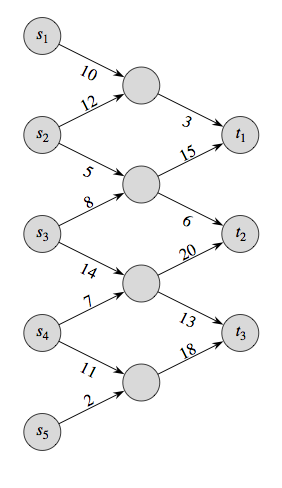
\includegraphics[height = 0.8\textheight]{Multi-source.png}
		\end{center}
	\end{frame}
	
	\begin{frame}
		\frametitle{Problema con múltiples fuentes o múltiples sumideros}
		Poner una súper fuente $s$ y súper sumidero $t$ que tengan capacidad infinita a las demás fuentes / sumideros y correr el algoritmo desde $s$ hasta $t$.
		\begin{center}
			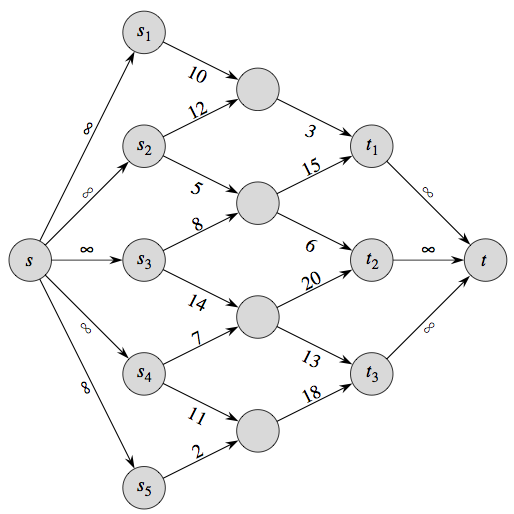
\includegraphics[height = 0.7\textheight]{Super-source.png}
		\end{center}
	\end{frame}
	
	\begin{frame}
		\frametitle{Problema donde los nodos también tienen capacidad}
		¿Qué hacer cuando, además de las aristas, los nodos también tienen una capacidad?
		\begin{figure}
			\begin{tikzpicture}[scale=1.8, auto,swap]
				\node[circle,fill=black!25,minimum size=30pt,inner sep=0pt] (s) at (0, 0.7) {$s$};
				\node[circle,fill=green!25,minimum size=30pt,inner sep=0pt] (a) at (1.5, 1.4) {$a/1$};
				\node[circle,fill=blue!25,minimum size=30pt,inner sep=0pt] (b) at (1.5, 0) {$b/2$};
				\node[circle,fill=red!25,minimum size=30pt,inner sep=0pt] (c) at (3, 0.7) {$c/5$};
				\node[circle,fill=black!25,minimum size=30pt,inner sep=0pt] (t) at (4.5, 0.7) {$t$};

				\foreach \source/ \dest /\weight in {s/b/6, b/c/9}
				\path[edge] (\source) -- node[weight] {$\weight$} (\dest);	
				\foreach \source/ \dest /\weight in {s/a/4, a/c/7, c/t/3}
				\path[edge] (\source) -- node[weight, above] {$\weight$} (\dest);
			\end{tikzpicture}
		\end{figure}
	\end{frame}
	
	\begin{frame}
		\frametitle{Problema donde los nodos también tienen capacidad}
		Dividir el nodo $u$ en 2: $u_1$ a donde llegan las aristas entrantes a $u$ y $u_2$ de donde salen las aristas salientes.\\
		Conectar $u_1$ y $u_2$ con una arista que tenga la misma capacidad que tenía el nodo $u$.
		\begin{figure}
			\begin{tikzpicture}[scale=1.8, auto,swap]
				\node[circle,fill=black!25,minimum size=30pt,inner sep=0pt] (s) at (0, 0.7) {$s$};
				
				\node[circle,fill=green!25,minimum size=20pt,inner sep=0pt] (a1) at (1.2, 1.4) {$a_1$};
				\node[circle,fill=green!25,minimum size=20pt,inner sep=0pt] (a2) at (1.9, 1.4) {$a_2$};
				
				\node[circle,fill=blue!25,minimum size=20pt,inner sep=0pt] (b1) at (1.2, 0) {$b_1$};
				\node[circle,fill=blue!25,minimum size=20pt,inner sep=0pt] (b2) at (1.9, 0) {$b_2$};
				
				\node[circle,fill=red!25,minimum size=20pt,inner sep=0pt] (c1) at (3, 0.7) {$c_1$};
				\node[circle,fill=red!25,minimum size=20pt,inner sep=0pt] (c2) at (3.7, 0.7) {$c_2$};
				
				\node[circle,fill=black!25,minimum size=30pt,inner sep=0pt] (t) at (5, 0.7) {$t$};

				\foreach \source/ \dest /\weight in {s/b1/6, b1/b2/2, b2/c1/9}
				\path[edge] (\source) -- node[weight] {$\weight$} (\dest);	
				\foreach \source/ \dest /\weight in {s/a1/4, a1/a2/1, a2/c1/7, c1/c2/5, c2/t/3}
				\path[edge] (\source) -- node[weight, above] {$\weight$} (\dest);
			\end{tikzpicture}
		\end{figure}
	\end{frame}
	
%\section[MBM]{Maximum Bipartite Matching}


\section{Tarea}
	\begin{frame}[fragile]
		\frametitle{Tarea}
		\begin{alertblock}{Tarea}
			Resolver los problemas de \url{http://contests.factorcomun.org/contests/59}
		\end{alertblock}
	\end{frame}
	
	\begin{frame}
		\frametitle{Ayuda}
		\begin{block}{Problema A}
			Ya son tan tesos que no necesitan ayuda para este problema :)
		\end{block}
		\begin{block}{Problema B}
			\begin{itemize}
				\item Hay que hallar el mínimo costo de cortar aristas o destruir nodos de manera que $s$ y $t$ queden desconectados.
				\item Ya sabemos que el mínimo corte de aristas es lo mismo que el máximo flujo
				\item ¿Cómo hacer para que los nodos también se tengan en cuenta para el corte?
				\item ¿Será que se puede hacer algo para que los nodos tengan implícitas aristas?
			\end{itemize}
		\end{block}
	\end{frame}

\end{document}